% Created by tikzDevice version 0.12.6 on 2024-11-11 09:19:14
% !TEX encoding = UTF-8 Unicode
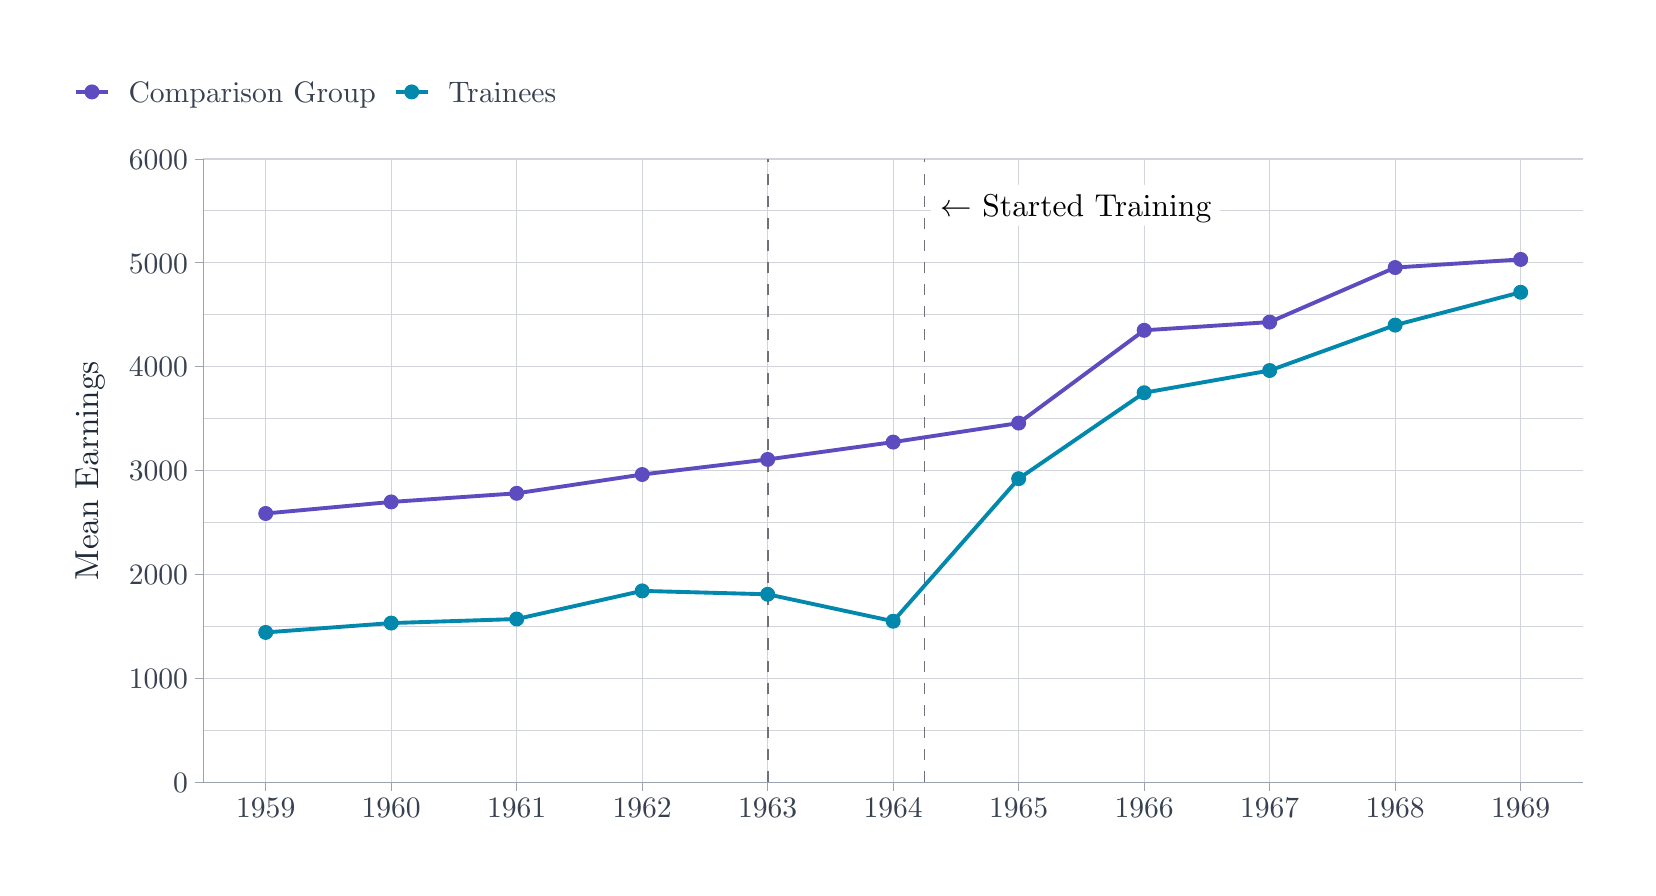
\begin{tikzpicture}[x=1pt,y=1pt]
\definecolor{fillColor}{RGB}{255,255,255}
\path[use as bounding box,fill=fillColor] (0,0) rectangle (578.16,303.53);
\begin{scope}
\path[clip] (  0.00,  0.00) rectangle (578.16,303.53);
\definecolor{drawColor}{RGB}{255,255,255}

\path[draw=drawColor,line width= 0.6pt,line join=round,line cap=round,fill=fillColor] (  0.00,  0.00) rectangle (578.16,303.53);
\end{scope}
\begin{scope}
\path[clip] ( 63.33, 30.82) rectangle (562.16,256.08);
\definecolor{drawColor}{RGB}{255,255,255}
\definecolor{fillColor}{RGB}{255,255,255}

\path[draw=drawColor,line width= 0.6pt,line join=round,line cap=round,fill=fillColor] ( 63.33, 30.82) rectangle (562.16,256.08);
\definecolor{drawColor}{RGB}{209,213,219}

\path[draw=drawColor,line width= 0.4pt,line join=round] ( 63.33, 49.59) --
	(562.16, 49.59);

\path[draw=drawColor,line width= 0.4pt,line join=round] ( 63.33, 87.14) --
	(562.16, 87.14);

\path[draw=drawColor,line width= 0.4pt,line join=round] ( 63.33,124.68) --
	(562.16,124.68);

\path[draw=drawColor,line width= 0.4pt,line join=round] ( 63.33,162.22) --
	(562.16,162.22);

\path[draw=drawColor,line width= 0.4pt,line join=round] ( 63.33,199.77) --
	(562.16,199.77);

\path[draw=drawColor,line width= 0.4pt,line join=round] ( 63.33,237.31) --
	(562.16,237.31);

\path[draw=drawColor,line width= 0.4pt,line join=round] ( 63.33, 30.82) --
	(562.16, 30.82);

\path[draw=drawColor,line width= 0.4pt,line join=round] ( 63.33, 68.37) --
	(562.16, 68.37);

\path[draw=drawColor,line width= 0.4pt,line join=round] ( 63.33,105.91) --
	(562.16,105.91);

\path[draw=drawColor,line width= 0.4pt,line join=round] ( 63.33,143.45) --
	(562.16,143.45);

\path[draw=drawColor,line width= 0.4pt,line join=round] ( 63.33,180.99) --
	(562.16,180.99);

\path[draw=drawColor,line width= 0.4pt,line join=round] ( 63.33,218.54) --
	(562.16,218.54);

\path[draw=drawColor,line width= 0.4pt,line join=round] ( 63.33,256.08) --
	(562.16,256.08);

\path[draw=drawColor,line width= 0.4pt,line join=round] ( 86.01, 30.82) --
	( 86.01,256.08);

\path[draw=drawColor,line width= 0.4pt,line join=round] (131.35, 30.82) --
	(131.35,256.08);

\path[draw=drawColor,line width= 0.4pt,line join=round] (176.70, 30.82) --
	(176.70,256.08);

\path[draw=drawColor,line width= 0.4pt,line join=round] (222.05, 30.82) --
	(222.05,256.08);

\path[draw=drawColor,line width= 0.4pt,line join=round] (267.40, 30.82) --
	(267.40,256.08);

\path[draw=drawColor,line width= 0.4pt,line join=round] (312.75, 30.82) --
	(312.75,256.08);

\path[draw=drawColor,line width= 0.4pt,line join=round] (358.09, 30.82) --
	(358.09,256.08);

\path[draw=drawColor,line width= 0.4pt,line join=round] (403.44, 30.82) --
	(403.44,256.08);

\path[draw=drawColor,line width= 0.4pt,line join=round] (448.79, 30.82) --
	(448.79,256.08);

\path[draw=drawColor,line width= 0.4pt,line join=round] (494.14, 30.82) --
	(494.14,256.08);

\path[draw=drawColor,line width= 0.4pt,line join=round] (539.49, 30.82) --
	(539.49,256.08);
\definecolor{drawColor}{RGB}{113,113,122}

\path[draw=drawColor,line width= 0.6pt,dash pattern=on 4pt off 4pt ,line join=round] (267.40, 30.82) -- (267.40,256.08);

\path[draw=drawColor,line width= 0.6pt,dash pattern=on 4pt off 4pt ,line join=round] (324.08, 30.82) -- (324.08,256.08);

\path[fill=fillColor] (328.41,232.00) --
	(428.87,232.00) --
	(428.79,232.00) --
	(429.12,232.02) --
	(429.44,232.08) --
	(429.75,232.20) --
	(430.04,232.37) --
	(430.29,232.58) --
	(430.51,232.82) --
	(430.69,233.10) --
	(430.82,233.41) --
	(430.90,233.73) --
	(430.93,234.06) --
	(430.93,234.06) --
	(430.93,244.64) --
	(430.93,244.64) --
	(430.90,244.97) --
	(430.82,245.29) --
	(430.69,245.59) --
	(430.51,245.87) --
	(430.29,246.12) --
	(430.04,246.33) --
	(429.75,246.50) --
	(429.44,246.61) --
	(429.12,246.68) --
	(428.87,246.69) --
	(328.41,246.69) --
	(328.65,246.68) --
	(328.32,246.69) --
	(328.00,246.65) --
	(327.68,246.56) --
	(327.38,246.42) --
	(327.11,246.23) --
	(326.87,246.00) --
	(326.67,245.74) --
	(326.52,245.44) --
	(326.41,245.13) --
	(326.36,244.80) --
	(326.35,244.64) --
	(326.35,234.06) --
	(326.36,234.22) --
	(326.36,233.89) --
	(326.41,233.57) --
	(326.52,233.25) --
	(326.67,232.96) --
	(326.87,232.70) --
	(327.11,232.47) --
	(327.38,232.28) --
	(327.68,232.14) --
	(328.00,232.04) --
	(328.32,232.00) --
	cycle;
\end{scope}
\begin{scope}
\path[clip] ( 63.33, 30.82) rectangle (562.16,256.08);
\definecolor{drawColor}{RGB}{0,0,0}

\node[text=drawColor,anchor=base west,inner sep=0pt, outer sep=0pt, scale=  1.14] at (329.78,235.43) {$\leftarrow$ Started Training};
\end{scope}
\begin{scope}
\path[clip] ( 63.33, 30.82) rectangle (562.16,256.08);
\definecolor{drawColor}{RGB}{1,136,172}
\definecolor{fillColor}{RGB}{1,136,172}

\path[draw=drawColor,line width= 0.4pt,line join=round,line cap=round,fill=fillColor] ( 86.01, 85.00) circle (  2.50);
\definecolor{drawColor}{RGB}{92,76,191}
\definecolor{fillColor}{RGB}{92,76,191}

\path[draw=drawColor,line width= 0.4pt,line join=round,line cap=round,fill=fillColor] ( 86.01,127.98) circle (  2.50);
\definecolor{drawColor}{RGB}{1,136,172}
\definecolor{fillColor}{RGB}{1,136,172}

\path[draw=drawColor,line width= 0.4pt,line join=round,line cap=round,fill=fillColor] (131.35, 88.38) circle (  2.50);
\definecolor{drawColor}{RGB}{92,76,191}
\definecolor{fillColor}{RGB}{92,76,191}

\path[draw=drawColor,line width= 0.4pt,line join=round,line cap=round,fill=fillColor] (131.35,132.15) circle (  2.50);
\definecolor{drawColor}{RGB}{1,136,172}
\definecolor{fillColor}{RGB}{1,136,172}

\path[draw=drawColor,line width= 0.4pt,line join=round,line cap=round,fill=fillColor] (176.70, 89.84) circle (  2.50);
\definecolor{drawColor}{RGB}{92,76,191}
\definecolor{fillColor}{RGB}{92,76,191}

\path[draw=drawColor,line width= 0.4pt,line join=round,line cap=round,fill=fillColor] (176.70,135.27) circle (  2.50);
\definecolor{drawColor}{RGB}{1,136,172}
\definecolor{fillColor}{RGB}{1,136,172}

\path[draw=drawColor,line width= 0.4pt,line join=round,line cap=round,fill=fillColor] (222.05,100.01) circle (  2.50);
\definecolor{drawColor}{RGB}{92,76,191}
\definecolor{fillColor}{RGB}{92,76,191}

\path[draw=drawColor,line width= 0.4pt,line join=round,line cap=round,fill=fillColor] (222.05,142.06) circle (  2.50);
\definecolor{drawColor}{RGB}{1,136,172}
\definecolor{fillColor}{RGB}{1,136,172}

\path[draw=drawColor,line width= 0.4pt,line join=round,line cap=round,fill=fillColor] (267.40, 98.78) circle (  2.50);
\definecolor{drawColor}{RGB}{92,76,191}
\definecolor{fillColor}{RGB}{92,76,191}

\path[draw=drawColor,line width= 0.4pt,line join=round,line cap=round,fill=fillColor] (267.40,147.51) circle (  2.50);
\definecolor{drawColor}{RGB}{1,136,172}
\definecolor{fillColor}{RGB}{1,136,172}

\path[draw=drawColor,line width= 0.4pt,line join=round,line cap=round,fill=fillColor] (312.75, 89.05) circle (  2.50);
\definecolor{drawColor}{RGB}{92,76,191}
\definecolor{fillColor}{RGB}{92,76,191}

\path[draw=drawColor,line width= 0.4pt,line join=round,line cap=round,fill=fillColor] (312.75,153.78) circle (  2.50);
\definecolor{drawColor}{RGB}{1,136,172}
\definecolor{fillColor}{RGB}{1,136,172}

\path[draw=drawColor,line width= 0.4pt,line join=round,line cap=round,fill=fillColor] (358.09,140.56) circle (  2.50);
\definecolor{drawColor}{RGB}{92,76,191}
\definecolor{fillColor}{RGB}{92,76,191}

\path[draw=drawColor,line width= 0.4pt,line join=round,line cap=round,fill=fillColor] (358.09,160.65) circle (  2.50);
\definecolor{drawColor}{RGB}{1,136,172}
\definecolor{fillColor}{RGB}{1,136,172}

\path[draw=drawColor,line width= 0.4pt,line join=round,line cap=round,fill=fillColor] (403.44,171.61) circle (  2.50);
\definecolor{drawColor}{RGB}{92,76,191}
\definecolor{fillColor}{RGB}{92,76,191}

\path[draw=drawColor,line width= 0.4pt,line join=round,line cap=round,fill=fillColor] (403.44,194.17) circle (  2.50);
\definecolor{drawColor}{RGB}{1,136,172}
\definecolor{fillColor}{RGB}{1,136,172}

\path[draw=drawColor,line width= 0.4pt,line join=round,line cap=round,fill=fillColor] (448.79,179.64) circle (  2.50);
\definecolor{drawColor}{RGB}{92,76,191}
\definecolor{fillColor}{RGB}{92,76,191}

\path[draw=drawColor,line width= 0.4pt,line join=round,line cap=round,fill=fillColor] (448.79,197.14) circle (  2.50);
\definecolor{drawColor}{RGB}{1,136,172}
\definecolor{fillColor}{RGB}{1,136,172}

\path[draw=drawColor,line width= 0.4pt,line join=round,line cap=round,fill=fillColor] (494.14,196.05) circle (  2.50);
\definecolor{drawColor}{RGB}{92,76,191}
\definecolor{fillColor}{RGB}{92,76,191}

\path[draw=drawColor,line width= 0.4pt,line join=round,line cap=round,fill=fillColor] (494.14,216.85) circle (  2.50);
\definecolor{drawColor}{RGB}{1,136,172}
\definecolor{fillColor}{RGB}{1,136,172}

\path[draw=drawColor,line width= 0.4pt,line join=round,line cap=round,fill=fillColor] (539.49,207.91) circle (  2.50);
\definecolor{drawColor}{RGB}{92,76,191}
\definecolor{fillColor}{RGB}{92,76,191}

\path[draw=drawColor,line width= 0.4pt,line join=round,line cap=round,fill=fillColor] (539.49,219.78) circle (  2.50);

\path[draw=drawColor,line width= 1.4pt,line join=round] ( 86.01,127.98) --
	(131.35,132.15) --
	(176.70,135.27) --
	(222.05,142.06) --
	(267.40,147.51) --
	(312.75,153.78) --
	(358.09,160.65) --
	(403.44,194.17) --
	(448.79,197.14) --
	(494.14,216.85) --
	(539.49,219.78);
\definecolor{drawColor}{RGB}{1,136,172}

\path[draw=drawColor,line width= 1.4pt,line join=round] ( 86.01, 85.00) --
	(131.35, 88.38) --
	(176.70, 89.84) --
	(222.05,100.01) --
	(267.40, 98.78) --
	(312.75, 89.05) --
	(358.09,140.56) --
	(403.44,171.61) --
	(448.79,179.64) --
	(494.14,196.05) --
	(539.49,207.91);
\end{scope}
\begin{scope}
\path[clip] (  0.00,  0.00) rectangle (578.16,303.53);
\definecolor{drawColor}{RGB}{156,163,175}

\path[draw=drawColor,line width= 0.3pt,line join=round] ( 63.33, 30.82) --
	( 63.33,256.08);
\end{scope}
\begin{scope}
\path[clip] (  0.00,  0.00) rectangle (578.16,303.53);
\definecolor{drawColor}{RGB}{55,65,81}

\node[text=drawColor,anchor=base east,inner sep=0pt, outer sep=0pt, scale=  1.07] at ( 57.93, 27.15) {0};

\node[text=drawColor,anchor=base east,inner sep=0pt, outer sep=0pt, scale=  1.07] at ( 57.93, 64.69) {1000};

\node[text=drawColor,anchor=base east,inner sep=0pt, outer sep=0pt, scale=  1.07] at ( 57.93,102.23) {2000};

\node[text=drawColor,anchor=base east,inner sep=0pt, outer sep=0pt, scale=  1.07] at ( 57.93,139.78) {3000};

\node[text=drawColor,anchor=base east,inner sep=0pt, outer sep=0pt, scale=  1.07] at ( 57.93,177.32) {4000};

\node[text=drawColor,anchor=base east,inner sep=0pt, outer sep=0pt, scale=  1.07] at ( 57.93,214.86) {5000};

\node[text=drawColor,anchor=base east,inner sep=0pt, outer sep=0pt, scale=  1.07] at ( 57.93,252.41) {6000};
\end{scope}
\begin{scope}
\path[clip] (  0.00,  0.00) rectangle (578.16,303.53);
\definecolor{drawColor}{RGB}{156,163,175}

\path[draw=drawColor,line width= 0.3pt,line join=round] ( 60.33, 30.82) --
	( 63.33, 30.82);

\path[draw=drawColor,line width= 0.3pt,line join=round] ( 60.33, 68.37) --
	( 63.33, 68.37);

\path[draw=drawColor,line width= 0.3pt,line join=round] ( 60.33,105.91) --
	( 63.33,105.91);

\path[draw=drawColor,line width= 0.3pt,line join=round] ( 60.33,143.45) --
	( 63.33,143.45);

\path[draw=drawColor,line width= 0.3pt,line join=round] ( 60.33,180.99) --
	( 63.33,180.99);

\path[draw=drawColor,line width= 0.3pt,line join=round] ( 60.33,218.54) --
	( 63.33,218.54);

\path[draw=drawColor,line width= 0.3pt,line join=round] ( 60.33,256.08) --
	( 63.33,256.08);
\end{scope}
\begin{scope}
\path[clip] (  0.00,  0.00) rectangle (578.16,303.53);
\definecolor{drawColor}{RGB}{156,163,175}

\path[draw=drawColor,line width= 0.3pt,line join=round] ( 63.33, 30.82) --
	(562.16, 30.82);
\end{scope}
\begin{scope}
\path[clip] (  0.00,  0.00) rectangle (578.16,303.53);
\definecolor{drawColor}{RGB}{156,163,175}

\path[draw=drawColor,line width= 0.3pt,line join=round] ( 86.01, 27.82) --
	( 86.01, 30.82);

\path[draw=drawColor,line width= 0.3pt,line join=round] (131.35, 27.82) --
	(131.35, 30.82);

\path[draw=drawColor,line width= 0.3pt,line join=round] (176.70, 27.82) --
	(176.70, 30.82);

\path[draw=drawColor,line width= 0.3pt,line join=round] (222.05, 27.82) --
	(222.05, 30.82);

\path[draw=drawColor,line width= 0.3pt,line join=round] (267.40, 27.82) --
	(267.40, 30.82);

\path[draw=drawColor,line width= 0.3pt,line join=round] (312.75, 27.82) --
	(312.75, 30.82);

\path[draw=drawColor,line width= 0.3pt,line join=round] (358.09, 27.82) --
	(358.09, 30.82);

\path[draw=drawColor,line width= 0.3pt,line join=round] (403.44, 27.82) --
	(403.44, 30.82);

\path[draw=drawColor,line width= 0.3pt,line join=round] (448.79, 27.82) --
	(448.79, 30.82);

\path[draw=drawColor,line width= 0.3pt,line join=round] (494.14, 27.82) --
	(494.14, 30.82);

\path[draw=drawColor,line width= 0.3pt,line join=round] (539.49, 27.82) --
	(539.49, 30.82);
\end{scope}
\begin{scope}
\path[clip] (  0.00,  0.00) rectangle (578.16,303.53);
\definecolor{drawColor}{RGB}{55,65,81}

\node[text=drawColor,anchor=base,inner sep=0pt, outer sep=0pt, scale=  1.07] at ( 86.01, 18.07) {1959};

\node[text=drawColor,anchor=base,inner sep=0pt, outer sep=0pt, scale=  1.07] at (131.35, 18.07) {1960};

\node[text=drawColor,anchor=base,inner sep=0pt, outer sep=0pt, scale=  1.07] at (176.70, 18.07) {1961};

\node[text=drawColor,anchor=base,inner sep=0pt, outer sep=0pt, scale=  1.07] at (222.05, 18.07) {1962};

\node[text=drawColor,anchor=base,inner sep=0pt, outer sep=0pt, scale=  1.07] at (267.40, 18.07) {1963};

\node[text=drawColor,anchor=base,inner sep=0pt, outer sep=0pt, scale=  1.07] at (312.75, 18.07) {1964};

\node[text=drawColor,anchor=base,inner sep=0pt, outer sep=0pt, scale=  1.07] at (358.09, 18.07) {1965};

\node[text=drawColor,anchor=base,inner sep=0pt, outer sep=0pt, scale=  1.07] at (403.44, 18.07) {1966};

\node[text=drawColor,anchor=base,inner sep=0pt, outer sep=0pt, scale=  1.07] at (448.79, 18.07) {1967};

\node[text=drawColor,anchor=base,inner sep=0pt, outer sep=0pt, scale=  1.07] at (494.14, 18.07) {1968};

\node[text=drawColor,anchor=base,inner sep=0pt, outer sep=0pt, scale=  1.07] at (539.49, 18.07) {1969};
\end{scope}
\begin{scope}
\path[clip] (  0.00,  0.00) rectangle (578.16,303.53);
\definecolor{drawColor}{RGB}{31,41,55}

\node[text=drawColor,rotate= 90.00,anchor=base,inner sep=0pt, outer sep=0pt, scale=  1.20] at ( 25.43,143.45) {Mean Earnings};
\end{scope}
\begin{scope}
\path[clip] (  0.00,  0.00) rectangle (578.16,303.53);
\definecolor{drawColor}{RGB}{255,255,255}
\definecolor{fillColor}{RGB}{255,255,255}

\path[draw=drawColor,line width= 0.6pt,line join=round,line cap=round,fill=fillColor] ( 16.00,268.08) rectangle (190.90,287.53);
\end{scope}
\begin{scope}
\path[clip] (  0.00,  0.00) rectangle (578.16,303.53);
\definecolor{drawColor}{RGB}{255,255,255}
\definecolor{fillColor}{RGB}{255,255,255}

\path[draw=drawColor,line width= 0.6pt,line join=round,line cap=round,fill=fillColor] ( 16.00,273.08) rectangle ( 30.45,287.53);
\end{scope}
\begin{scope}
\path[clip] (  0.00,  0.00) rectangle (578.16,303.53);
\definecolor{drawColor}{RGB}{92,76,191}
\definecolor{fillColor}{RGB}{92,76,191}

\path[draw=drawColor,line width= 0.4pt,line join=round,line cap=round,fill=fillColor] ( 23.23,280.31) circle (  2.50);
\end{scope}
\begin{scope}
\path[clip] (  0.00,  0.00) rectangle (578.16,303.53);
\definecolor{drawColor}{RGB}{92,76,191}

\path[draw=drawColor,line width= 1.4pt,line join=round] ( 17.45,280.31) -- ( 29.01,280.31);
\end{scope}
\begin{scope}
\path[clip] (  0.00,  0.00) rectangle (578.16,303.53);
\definecolor{drawColor}{RGB}{255,255,255}
\definecolor{fillColor}{RGB}{255,255,255}

\path[draw=drawColor,line width= 0.6pt,line join=round,line cap=round,fill=fillColor] (131.54,273.08) rectangle (146.00,287.53);
\end{scope}
\begin{scope}
\path[clip] (  0.00,  0.00) rectangle (578.16,303.53);
\definecolor{drawColor}{RGB}{1,136,172}
\definecolor{fillColor}{RGB}{1,136,172}

\path[draw=drawColor,line width= 0.4pt,line join=round,line cap=round,fill=fillColor] (138.77,280.31) circle (  2.50);
\end{scope}
\begin{scope}
\path[clip] (  0.00,  0.00) rectangle (578.16,303.53);
\definecolor{drawColor}{RGB}{1,136,172}

\path[draw=drawColor,line width= 1.4pt,line join=round] (132.99,280.31) -- (144.55,280.31);
\end{scope}
\begin{scope}
\path[clip] (  0.00,  0.00) rectangle (578.16,303.53);
\definecolor{drawColor}{RGB}{55,65,81}

\node[text=drawColor,anchor=base west,inner sep=0pt, outer sep=0pt, scale=  1.07] at ( 36.45,276.63) {Comparison Group};
\end{scope}
\begin{scope}
\path[clip] (  0.00,  0.00) rectangle (578.16,303.53);
\definecolor{drawColor}{RGB}{55,65,81}

\node[text=drawColor,anchor=base west,inner sep=0pt, outer sep=0pt, scale=  1.07] at (152.00,276.63) {Trainees};
\end{scope}
\end{tikzpicture}
